Previous work of visual transfer learning focuses on designing classifiers that can leverage the source knowledge effectively. In this section, we briefly review methods for the visual transfer learning and show the limitation of previous work. 
\subsection{Intuition for Visual Transfer Learning}
The intuition of visual transfer learning comes from human recognition mechanism. For our human, all the information acquired is stored in our memory. This information is organized according to the properties. When we see a new concept, we don't treat it isolated but connect it to certain previous knowledge we stored in our memory. By comparing a new concept with the organized information in our memory, we can capture the property of a new concept effectively. When referring to visual tasks, several examples can be given to show this cognitive ability. For instance, when we describe the animal "okapi" (see Figure \ref{fig:intro:multi}), we would probably say that: okapi has a body of a horse, legs of the zebra and the head of giraffe. People who never see a zebra could instantly have a rough idea of a zebra. 

\begin{figure}
	\centering
	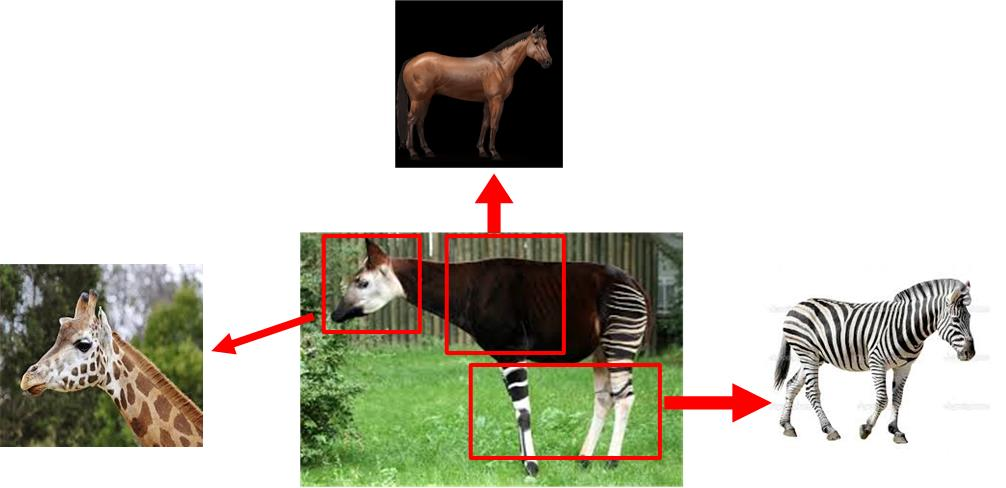
\includegraphics[scale=.6]{introduction/fig/multiple.jpg}
	\caption{An intuitive description for human to learn new concept: an okapi can be roughly described as the combination of a body of a horse, legs of the zebra and a head of giraffe.}\label{fig:intro:multi}
\end{figure}

This indicates that to learn a concept effectively, we should be able to make use of the gained knowledge instead of learning it from scratch. This process is commonly referred to as transfer learning\cite{pan2010survey}. Traditional machine learning methods work under the common assumption: training data and testing data are drawn from the same feature space and same distribution. 
In transfer learning, the test data can come from a different distribution. The data from the original distribution is called source data, and data from the new distribution is called target data. Transfer learning is used to utilize the source knowledge from the source data to help to build the new model to classify the target data. 

\subsection{Approaches for Visual Transfer Learning}
Successfully leveraging the source knowledge can greatly improve the performance of the target model. In general, the more related the source and target domain are, the more useful the source knowledge is and the more benefit the target model can get. Leveraging unrelated knowledge cannot help to improve the performance of the target model or even hurt it. Therefore, the key issue for visual transfer learning is to identify the relatedness of the source and target domain. The major approach for Visual Transfer Learning consists of two main directions: Distribution Similarity Measurement and Instance Reuse.

\begin{itemize}
	\item \textbf{Distribution Similarity Measurement}. The core idea of transfer learning is to leverage the related source knowledge. The more related the source is, the better transfer performance we can achieve. Thus, measuring the relatedness of the source knowledge is an important part in transfer learning especially where there are multiple sources. A straight-forward approach to identify the relatedness of the source and target domain is to measure their similarity directly. Measuring the data discrepancy through some statistical measurements such as \textbf{Maximum Mean Discrepancy} (MMD) \cite{duan2009domain}, has been a popular way to identify the source and target domain. MMD reflects the distance of two data distributions in the Reproducing Kernel Hilbert Space (RKHS) \cite{aronszajn1950theory}.
	\item \textbf{Instance Reuse}\cite{lim2012transfer}. We apply transfer learning under the scenario where the target data is scarce and we are not able to build the target model alone with the target data. A simple solution is to ``borrow" some of the data from the source domain and use it to build the target model together with the target data. This approach can directly increase the size of the data in the target domain and effectively improve the performance of the target model. For example, \textbf{Feature Transformation} \cite{duan2012learning} can overcome the data distribution mismatch in different domains and project the data into the same augmented space and thus can increase the training data for the target task as well (see Figure \ref{fig:intro:trans}).
\end{itemize}

\begin{figure}
	\centering
	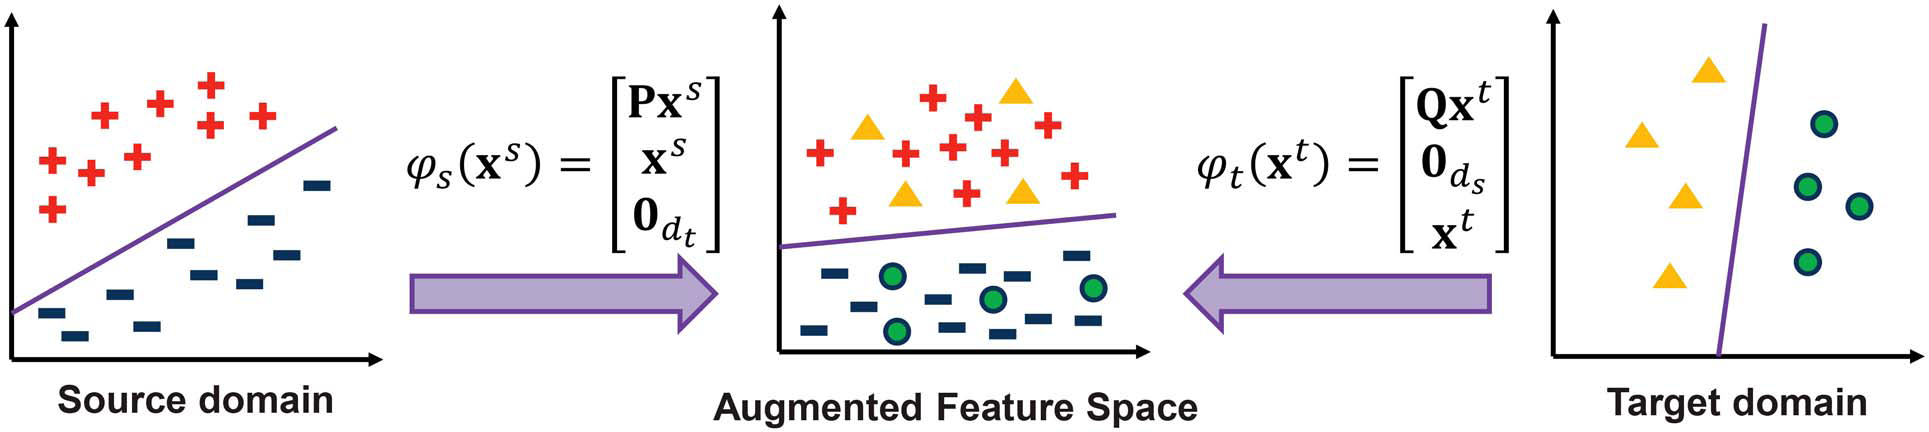
\includegraphics[scale=.3]{introduction/fig/transformation.png}
	\caption{Feature transformation. Transform the data in different domains into a augmented feature space.}\label{fig:intro:trans}
\end{figure}

\subsection{Limitation of Previous Methods}
From the review of the approaches for Visual Transfer Learning we can see that
most previous methods require access to the source data to obtain the source knowledge. However, in many practical problems, these previous approaches may not be as convenient as we thought due to the following reasons:

\begin{itemize}
	\item \textbf{Data accessibility}. The source data may not be able to access for some tasks. For example, the clinical database is not allowed to access for general publics due to the privacy. Disclosure obligations and will to share the databases are also two important reasons that make the source data inaccessible.
	\item \textbf{Size of the source data}. Besides data accessibility, many previous methods \cite{daume2009frustratingly}\cite{duan2012learning} require accessing to each of the individual source instance to obtain the source knowledge which is ineffective for many large source domain. For example, it is almost impossible to measure the MMD for some large source domain which contains hundreds of thousands of instances.
\end{itemize}

From above we can see that these previous methods can successfully leverage the source knowledge under the assumption that the source data are freely accessible and relatively small. However, this assumption could fail in real applications. In some cases, the source data could be private (such as the clinic data from patients) and therefore, could not be shared with the public. Moreover, those large source dataset contains more knowledge and information compared to the small ones and thus can better improve the transfer performance of the target task. However, obtaining the similarity measurement of these large datasets with those previous methods can be tedious and inefficient. It is important to find a way to leverage the source knowledge without accessing to the source data.

In this thesis, we assume that we can freely access to the source model trained from the source data and thus leverage the knowledge from the model instead. Using the source model for transfer learning can successfully avoid the two issues discussed above. Source model can contain as much knowledge as the source data while without containing any information regarding the individual instance. Therefore, the owner of the source data does not have to worry about the data privacy issue. For those large source dataset such as ILSVRC containing millions of images, a trained source model is normally a few hundreds megabytes and public available. Therefore, leveraging the source knowledge from source model instead of the source data is more practical for real visual transfer learning applications.
%%%%%%%%%%%%%%%%%%%%%%%%%%%%%%%%%%%%%%%%%%%%%%%%%%%%%%%%%%%%%%%%%%%%%%%%%%%%%%%%%
